\documentclass[french]{article}
\usepackage[T1]{fontenc}
\usepackage[utf8]{inputenc}
\usepackage{lmodern}
\usepackage[a4paper]{geometry}
\usepackage{babel}
\usepackage{listings}             % Include the listings-package
\usepackage{amsfonts}
\usepackage{color}
\usepackage{stmaryrd}

\usepackage{tikz}
\usepackage{tikz-qtree}

\definecolor{mygreen}{rgb}{0,0.6,0}
\definecolor{mygray}{rgb}{0.5,0.5,0.5}
\definecolor{mymauve}{rgb}{0.58,0,0.82}

\lstset{ %
  backgroundcolor=\color{white},   % choose the background color; you must add \usepackage{color} or \usepackage{xcolor}; should come as last argument
  basicstyle=\footnotesize,        % the size of the fonts that are used for the code
  breakatwhitespace=false,         % sets if automatic breaks should only happen at whitespace
  breaklines=true,                 % sets automatic line breaking
  captionpos=b,                    % sets the caption-position to bottom
  commentstyle=\color{mygreen},    % comment style
  deletekeywords={...},            % if you want to delete keywords from the given language
  escapeinside={\%*}{*)},          % if you want to add LaTeX within your code
  extendedchars=true,              % lets you use non-ASCII characters; for 8-bits encodings only, does not work with UTF-8
  frame=single,	                   % adds a frame around the code
  keepspaces=true,                 % keeps spaces in text, useful for keeping indentation of code (possibly needs columns=flexible)
  keywordstyle=\color{blue},       % keyword style
  language=Python,                 % the language of the code
  morekeywords={*,...},            % if you want to add more keywords to the set
  numbers=left,                    % where to put the line-numbers; possible values are (none, left, right)
  numbersep=5pt,                   % how far the line-numbers are from the code
  numberstyle=\tiny\color{mygray}, % the style that is used for the line-numbers
  rulecolor=\color{black},         % if not set, the frame-color may be changed on line-breaks within not-black text (e.g. comments (green here))
  showspaces=false,                % show spaces everywhere adding particular underscores; it overrides 'showstringspaces'
  showstringspaces=false,          % underline spaces within strings only
  showtabs=false,                  % show tabs within strings adding particular underscores
  stepnumber=2,                    % the step between two line-numbers. If it's 1, each line will be numbered
  stringstyle=\color{mymauve},     % string literal style
  tabsize=2,	                   % sets default tabsize to 2 spaces
  title=\lstname                   % show the filename of files included with \lstinputlisting; also try caption instead of title
}

\title{Recherche des structures secondaires d’une chaîne d’ADN\\
\large Projet 2I003}
%\title{Recherche des structures secondaires d’une chaîne d’ADN}
\author{LI Mengda, GE Zhichun}


\begin{document}
\lstset{language=Python}	

\maketitle

\section{Exercice 1}

\subsection{}
\label{subsec:q1}
Comme un nucléotide ne peut former une paire avec lui même, donc 

\begin{center}
$\forall i\in\{1,...,n\}, \quad S_{i,i} = \{\}$ et $ E_{i,i} = 0$
\par\end{center}

\subsection{}
\label{subsec:q2}

	\subsubsection{}
	Si ni i, ni j ne sont couplés dans S$_{i,j}$ , alors
	%{\centering S$_{i,j}$ = S$_{i+1,j-1}$\par}
	\begin{center}
	$S_{i,j} = S_{i+1,j-1}$ \quad $E_{i,j} = E_{i+1,j-1}$
	\par\end{center}

	\subsubsection{}
	Si j n'est pas couplée dans S$_{i,j}$ , alors
	\[
	S_{i,j} = S_{i,j-1} \quad E_{i,j} = E_{i,j-1}
	\]

	\subsubsection{}
	Si $\left(i,j\right)\in S_{i,j}$, alors
	\[
	S_{i,j}   = S_{i+1,j-1}\, \cup \, \left(i,j\right) \quad  E_{i,j} = E_{i+1,j-1}+ 1
	\]

	\subsubsection{}
	Si $\left(k,j\right)\in S_{i,j}$ avec $k\in\left\{ i+1,...,j-1\right\} $, alors
	\[
	S_{i,j}= S_{i,k-1}\cup S_{k,j} \quad E_{i,j} = E_{i,k-1} + E_{k,j} 
	\]
	car, par hypothèse, il n'existe pas de nœud: lorsqu'on coupe en k, on ne coupe pas de couple dans ce cas là, il n'y a donc pas de perte. Sinon, on a $S_{i,j} \subset S_{i,k-1}\cup S_{k,j} $ dans tous les cas.
\subsection{}
\label{subsec:q3}
	\subsubsection{}

		Par la question \ref{subsec:q2}, résumons en distinguant tous les cas possibles:
\\
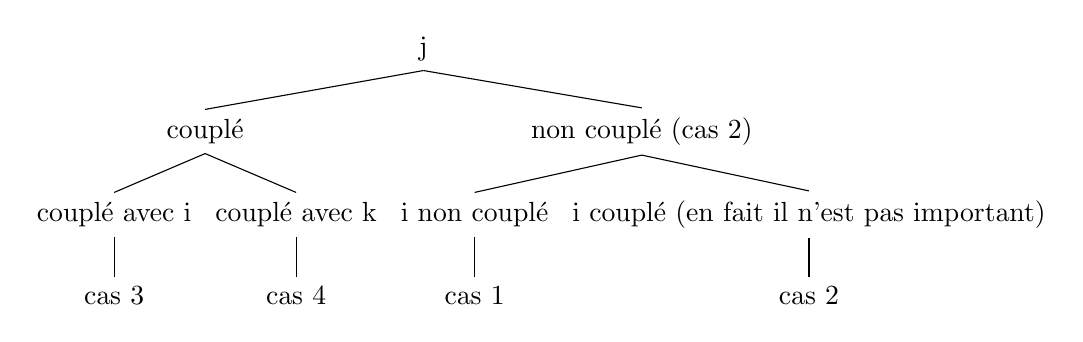
\begin{tikzpicture}
\Tree 
[.j	[.couplé 
			[.{couplé avec i} {cas 3} ]    [.{couplé avec k} {cas 4} ] 
	]
	[.{non couplé (cas 2)} 
			[.{i non couplé} {cas 1} ]	[.{i couplé (en fait il n'est pas important)} {cas 2} ]
	]
]

\end{tikzpicture}	
		\begin{enumerate}  
		\item \label{itm:1}
			 Soit ni i, ni j ne sont couplés dans S$_{i,j}$ , alors E$_{i,j}$ = E$_{i+1,j-1}$, \\
			et on a toujours E$_{i,j} \geq E_{i+1,j-1}$ dans tous les cas.
		\item Soit j n'est pas couplée dans S$_{i,j}$ , alors  E$_{i,j}$ = E$_{i,j-1}$, \\
			et on a toujours E$_{i,j} \geq E_{i,j-1}$ dans tous les cas.
	%	\item Soit i n'est pas couplée dans S$_{i,j}$ , alors  E$_{i,j}$ = E$_{i+1,j}$
		\item Soit j est couplé avec i, c'est à dire $\left(i,j\right)\in S_{i,j}$, alors E$_{i,j}$  = E$_{i+1,j-1}+1$
		\item Soit j est couplé avec un $k\in\left\{ i+1,...,j-1\right\} $, alors $E_{i,j} = E_{i,k-1} + E_{k,j}$,\\ sinon $E_{i,j} \geq E_{i,k-1} + E_{k,j}$ car $S_{i,j} \supset \, S_{i,k-1}\cup S_{k,j}\quad \forall k \in\left\{ i+1,...,j-1\right\}$
		\end{enumerate}
		
		Soit la fonction e :$ \{1, ... , n\} \times{} \{1, ... , n\} \rightarrow{} \{0, 1\}$ qui vaut 1 ssi i et j peuvent être couplés. \par
		\begin{description}
		\item
		\underline{Dans le cas  \ref{itm:1} et cas 3, $E_{i,j} = E_{i+1,j-1} + e(i,j)$ }  
et on a  \underline{$E_{i,j} \geq E_{i+1,j-1} + e(i,j)$ dans tous les cas. } 
			\begin{itemize} 
			\item si j est couplé avec i, $ e(i,j) = 1$, E$_{i,j}  = E_{i+1,j-1}+1 = E_{i+1,j-1}+ e(i,j) $, 
			\item sinon $ e(i,j) = 0$, on a toujours E$_{i,j} \geq E_{i+1,j-1} = E_{i+1,j-1}+ e(i,j)$ par le \ref{itm:1}.
			\end{itemize}	
		\item
		\underline{Dans le cas 2, $E_{i,j} = E_{i,j-1}$} et on a \underline{$E_{i,j} \geq E_{i,j-1}$ dans tous les cas.} car S$_{i,j} \supset S_{i,j-1}$
		\item
		Par le cas 4, $\forall k \in\left\{ i+1,...,j-1\right\} \; E_{i,j} \geq E_{i,k-1} + E_{k,j}$. Donc \underline{ $E_{i,j} \geq  \displaystyle \max_{i<k<j}  E_{i,k-1} + E_{k,j}$ dans tous les cas}.
		\\Et
		s'il existe $k_{0}\in\left\{ i+1,...,j-1\right\}$ tel que  $\left(k_{0},j\right)\in S_{i,j}$, $E_{i,j} = E_{i,k_{0}-1} + E_{k_{0},j}$\\
		Dans ce cas-là, le max est atteint:\\
		 $E_{i,k_{0}-1} + E_{k_{0},j} \geq  \displaystyle \max_{i<k<j}  E_{i,k-1} + E_{k,j}$ et $ \displaystyle \max_{i<k<j}  E_{i,k-1} + E_{k,j} \geq  E_{i,k_{0}-1} + E_{k_{0},j}$\\
		D'où \underline{ $E_{i,j} = E_{i,k_{0}-1} + E_{k_{0},j} = \displaystyle \max_{i<k<j}  E_{i,k-1} + E_{k,j}$ dans le cas 4}
		\end{description}
		En conclusion: $E_{i,j}$ est un majorant de l'ensemble $\{E_{i+1,j-1} + e(i,j), \, E_{i,j-1}, \,  \displaystyle \max_{i<k<j}  E_{i,k-1} \}$, et ce majorant est atteint: il y a toujours un cas où la condition d'égalité est vrai. 
		Donc
\begin{center}
 $E_{i,j} =\max\{E_{i+1,j-1} + e(i,j), \, E_{i,j-1}, \,  \displaystyle \max_{i<k<j}  E_{i,k-1} + E_{k,j}\}$
\par\end{center}
		...
	\subsubsection{}
	Si k = j, $ E_{k,j}=E_{j,j}=0$ par \ref{subsec:q1}, donc $E_{i,j-1}=(E_{i,j-1}+E_{j,j})\in \{E_{i,k-1} + E_{k,j} \mid i<k\leq j   \} $, et 
\begin{center}
$E_{i,j-1}\leq \max \{E_{i,k-1} + E_{k,j} \mid i<k\leq j   \} $
\par\end{center}

\begin{center}
On en déduit que $E_{i,j} =\max\{E_{i+1,j-1} + e(i,j), \,   \displaystyle \max_{i<k \leq j}  E_{i,k-1} + E_{k,j}\}$
\par\end{center}

\pagebreak
\subsection{}
	\begin{lstlisting}[frame=single]  % Start your code-block

def tailleMaxRec(a: str, i: int, j: int) -> int:
    n= len(a)
    assert 1 <= i <= n and 1 <= j <= n, 'impossible de tronquer'
    
    if a == '' or i >= j:
        return 0

    def couple(i: int, j:int) -> bool:
        return {a[i-1], a[j-1]} in [ {'A','T'}, {'C','G'} ]
    
    def e(i: int, j: int) -> {0,1}:
        if couple(i,j):
            return 1
        else:
            return 0

    return max(tailleMaxRec(a, i+1, j-1) + e(i,j),
               max([tailleMaxRec(a, i, k-1) + tailleMaxRec(a, k, j)
                    for k in range(i+1, j+1)]) )
	\end{lstlisting}


\subsection{}
Cette fonction se termine car chaque fois on appelle récursivement sur une sous-partie de séquence [i+1, j-1], le début de sous-séquence i est strictement croissant et la fin de sous-séquence j est stricetement décroissante. Dans $\mathbb{N}$, l'ordre est bien fondé donc i, j se rencontre en certaine récursion. Lorsque i, j se rencontre, c'est à dire $i \leq j$, la fonction retourne une valeure et se termine en dépillant récursivement.
\par
Cette fonction calcule exactement $\max\{E_{i+1,j-1} + e(i,j), \,    \max_{i<k<j}  E_{i,k-1} + E_{k,j}\}$, elle est valide selon la question \ref{subsec:q3}.

\subsection{}
\subsubsection{}
Pour $u_{0}$, $(p = 0) \Rightarrow (i = j)$. Donc l'appel de fonction retourne simplement 0, $u_{0}=1$ \par
Pour $u_{1}$, $(p = 1) \Rightarrow (i + 1 = j)$, donc cet appel retourne 
\begin{lstlisting}
max(tailleMaxRec(a, i+1, j-1) + e(i,j),
               max([tailleMaxRec(a, i, k-1) + tailleMaxRec(a, k, j)
                    for k in range(i+1, j+1)]) )\end{lstlisting}
Vu que i + 1 = j,  tailleMaxRec(a, i+1, j-1) retourne simplement 0 car $i+1=j\geq j-1$.\\
Analysons la dernière itérable 
\begin{lstlisting}
[tailleMaxRec(a, i, k-1) + tailleMaxRec(a, k, j) for k in range(i+1, j+1)]\end{lstlisting}
range(j ,j+1) ne contient que j, donc cette liste n'a qu'un élément, cela vaut dire qu'on appelle deux fois  \lstinline{tailleMaxRec}.
En sommant, $u_{1} = 3$
\subsubsection{}

Soit $p \leq 2$, pour $u_{p}$\\
	\begin{itemize}
	\item
	On appelle d'abord une fois la fonction elle-même: \lstinline{tailleMaxRec(a, i, j)}, on a 1 appel. 
	\item
	Et puis on appelle  \lstinline{ tailleMaxRec (a, i+1, j-1) },\\
	 $(j-1)-(i+1)=(j-i)-2=0$, on a donc $u_{0}$ appel(s).
	\item
	Enfin, pour \begin{lstlisting}
	tailleMaxRec(a,i,k-1) + tailleMaxRec(a,k,j) for k in range(i+1, j+1)\end{lstlisting}
	\lstinline{range(i+1, j+1)} équivaut à $\llbracket i+1, i+p \rrbracket$, car p = j - i, j = i + p\\
Le nombre d'appel de \lstinline{tailleMaxRec(a, i, k-1)} équivaut $u_{k-1-i}$,\\Le nombre d'appel de \lstinline{tailleMaxRec(a, k, j)} équivaut $u_{p+i-k}$\\	
On a donc $\sum_{k=i+1}^{i+p} u_{k-1-i} + \sum_{k=i+1}^{i+p} u_{p+i-k}$ d'appels.\\
Pour la première, en éffectuant un changement de variable q = k- (i+1), on a bien $\sum_{q=0}^{p-1} u_{q}$\\
Pour la deuxième, en éffectuant un changement de variable q = p + i - k, on a  $\sum_{q=p-1}^{0} u_{q}$ qui vaut en effet $\sum_{q=0}^{p-1} u_{q}$.\\
En sommant les deux sommes, on a bien $2\sum_{i=0}^{p-1} u_{i}$
	\end{itemize}
\par
En conclusion, $u_{p}=u_{0}+1+2\sum_{i=0}^{p-1} u_{i}$




\end{document}
Induction:
Soit $n \in \mathbb{N}, n\geq2 $ fixé, supposons $u_{n} = u_{0} + 1 + 2\sum_{i=0}^{1} u_{i}$
supposons $u_{k} = u_{k-2} + 1 + 2\sum_{i=0}^{k-1} u_{i}$
Démontrons par récurrence  le nombre d'appel de cette partie vaut $2\sum_{i=0}^{p-1} u_{i}$
		\begin{itemize}
		\item 
		Cas de base, p = 2, \lstinline{range(i+1, j+1)} équivaut à $\llbracket i+1, i+2 \rrbracket$, j = i +2
			\begin{description}
			\item
			Lorsque k = i + 1,\\
			on appelle \lstinline{tailleMaxRec(a, i, i)}, on a $u_{0}$ appel(s) et \\
			on appelle \lstinline{tailleMaxRec(a, i + 1, i + 2)}, on a $u_{1}$ appel(s)
			\item
			Lorsque k = i + 2,\\
			on appelle \lstinline{tailleMaxRec(a, i, i + 1)}, on a $u_{1}$ appel(s) et \\
			on appelle \lstinline{tailleMaxRec(a, i + 2, i + 2)}, on a $u_{0}$ appel(s)
			\end{description}
		On a bien  $ 2\sum_{i=0}^{1} u_{i}$ appels. \\\par
		\item
		Induction: Soit $n \in \mathbb{N}, n\geq2 $ fixé, supposons on a $2\sum_{i=0}^{n-1} u_{i}$ appels en $\llbracket i+1, i+n \rrbracket$ lorsque p = n. Notons P(n) le nombre d'appel sur $\llbracket i+1, i+n \rrbracket$.\\
Lorsque p = n + 1, $\llbracket i+1, i+n+1 \rrbracket= \llbracket i+1, i+n \rrbracket \cup \{n+1\}$, donc \begin{center} P(n+1) = P(n) + le nombre d'appel lorsque k = n+1 \end{center}	
		Lorsque k = n + 1,\\
		on appelle \lstinline{tailleMaxRec(a, i, n)}, on a $u_{n-i}$ appel(s) et \\
		on appelle \lstinline{tailleMaxRec(a, n + 1, i + n + 2)}, on a $u_{i+2}$ appel(s)	

	\end{itemize}